\documentclass{article}
\usepackage{../tex/mysty}
\geometry{left=1.5in}
\usepackage[final]{pdfpages}
\begin{document}


\maketitlepage{U.S. Food and Drug Administration: Regulatory
  Report}{Sanjay Challa}

\setcounter{tocdepth}{3}
\tableofcontents
\newpage

\section*{Executive summary}
\label{sec:exec-summary}
This focus of this document is on relevant FDA regulation of the
device our team has designed. The first section of this document
provides a general overview of FDA regulation of medical devices. The
FDA regulatory overview covers device classes, filing requirements for
510(k) and IDE/PMAs, and the meanings of FDA \textit{clearance} and
FDA \textit{approval}. The second section of this document covers FDA
regulation specific to our device. In this document, we explain that
the FDA currently does not regulate our device. We further outline
that since our device is meant only for use in research settings, does
not come into contact with patients, and is not used for diagnosis or
treatment, our device should not be regulated by the FDA. Our device
is simply a laboratory device intended for measurement purposes. While
there are a few standards from the FD \& C act which may apply to our
device, the primary performance standard of our device derives
directly from our client's needs and our design specifications. The
appendix of this document contain a mock Traditional 510(k) for our
device. In preparing the Traditional 510(k), we assumed that our
device was regulated as a Class II device by the FDA, and did our best
to draft the 510(k) under this premise. There are a number of elements
of the 510(k) which were trivial in relation to our device as our
device is not currently regulated by the FDA. 

\newpage
\section{Regulation Overview}
\label{sec:test-administration}

Medical devices are classified into Class I, II, and III based on the
level of regulatory control required by the FDA. All devices must
comply with the Class I General Controls. These include annual
establishment registration, or registration of owners and operators of
facilities that are involved in the production and distribution of
medical devices, as well as a medical device listing of all products
produced at a certain establishment. Devices must be made in
accordance with current good manufacturing practices (cGMPs), and
manufacturers must develop a system of quality control that in line
with any FDA quality systems (QS) guidelines applicable to their
device. All manufacturing processes and procedures must be
documented. The labeling on the device, including the claims and
advertising, should be in accordance with FDA regulations; it should
be clear, should not be misleading, and should not omit any required
important warnings. Finally, as required by FDA Medical Device
Reporting regulations, medical device manufacturers must report to the
FDA any complaints of malfunction of medical devices as well as
serious injuries or deaths associated with medical devices.

Class II products are defined as products for which general controls
alone are insufficient to assure safety and effectiveness.” Orthopedic
and craniofacial implants are Class II products, as opposed to manual
wheelchairs and hand-held surgical instruments, which are Class I
products.  In addition to following Class I General Controls, Class II
products are subject to Standards or Guidance Documents such as ASTM
or ISO Standards or OCD and OCER Guidance.

For Class II products, manufacturers or companies must submit a
premarket notification in the form of a 510(k). A 510(k) submission
requires the device name, the establishment registration number, the
device classification, documentation of performance standards, and
proposed labels and advertisements, as described in Class I General
Controls. In addition, a 510(k) submission requires a description of
“predicate devices” – devices already in the market that are similar
to the proposed product – and a statement detailing the similarities
and differences between predicate devices and the proposed
device. 510(k) clearance is based on substantial equivalency, which
means that “the new device is at least as safe and effective as the
predicate.” Predicate devices may be in any of the three device
classes. A product is substantially equivalent if it has the same
intended use and technological characteristics as the predicate
device. If a device has the same intended use as the predicate but
different technological characteristics, it should be proven to be as
safe and effective as the predicate and should not raise any new
safety issues.

Class III products are defined as those which “support or sustain
human life, are of substantial importance in preventing impairment of
human health, or which present a potential, unreasonable risk of
illness or injury.” A Pre-Market Approval (PMA) submission and, in
some cases, an investigational device exemption (IDE) are required for
approval of Class III devices. (An IDE may also be required for some
Class II product clearances). An IDE allows the investigational device
to be used in a clinical study, approved both by the FDA and an
Institutional Review Board, to collect safety and effectiveness data
required for a PMA.  In contrast to Class II devices, Class III
devices must receive FDA approval instead of clearance for their use,
components, and manufacturing methods. Class III devices are
significantly different from devices already existent on the market
and present new safety concerns that have not been tested. PMAs must
not only comply with Class I General Controls, but must also
demonstrate the safety and effectiveness of the device and include
both good science and scientific writing.
	 

\section{Device Classification}
\label{sec:protocols}

Searches in the \textit{FDA Product Classification Database} using the
keywords ``tomography,'' ``ophthalmic,'' and ``micrometer'' were
performed. A few entries were returned which related to our device:

\begin{enumerate}
\item Optical coherence tomography: General \& Plastic Surgery panel,
  regulation number 886.1570, product code OBO; describes an
  ophthalmoscope as an "Diagnostic device to aid in the detection and
  management of various ocular diseases" capable of "viewing, imaging,
  measurement, and analysis of ocular structures."
\item System, x-ray, tomography, computed: Radiology panel, regulation
  number 892.1750, product code JAK; describes a diagnostic x-ray
  system which relies upon similar technical principles as our
  device. The similarity lies in the method by which measurement
  slices are taken, and the manner in which measurement slices are
  combined to create a reconstruction.
\item Micrometers, Microscope: Pathology panel, regulation number
  864.3600, product code KEH; describes a microscopes and accessories
  as optical instruments used to enlarge images of specimens,
  preparations, and cultures for medical purposes.
\end{enumerate}

While the devices listed above share some common elements with our
device, none of the devices fully capture the intended use and
functionality of our device. One key difference between our device and
those listed above is that our device is not intended for any
diagnostic or clinical applications, but is instead targeted at
research applications. In this regard, our device is most likely not
regulated by the FDA as medical device. According to the FD\&C Act
21USC321, a "device" is "an instrument, apparatus, implement, machine,
contrivance, implant, in vitro reagent, or other similar or related
article, including any component, part, or accessory, which is:

\begin{itemize}
\item recognized in the official National Formulary, or the United
  States Pharmacopeia, or any supplement to them,
\item intended for use in the diagnosis of disease or other
  conditions, or in the cure, mitigation, treatment, or prevention of
  disease, in man or other animals, or
\item intended to affect the structure or any function of the body of
  man or other animals, and which does not achieve its primary
  intended purposes through chemical action within or on the body of
  man or other animals and which is not dependent upon being
  metabolized for the achievement of its primary intended purposes."
\end{itemize}

Our device clearly does not fall within any of the elements of the
above definition. It is not listed in the National Formulary, US
Pharmacopeia, nor any supplements to them. Furthermore, our device is
not intended for the diagnosis of disease or other conditions, or in
the cure, mitigation, treatment, or prevention of disease, in man or
other animals. It is solely intended for the measurement of eyeballs
dissected out of mice in research settings. Lastly, our device is not
intended for and does not affect the structure or functionality of
any man or animal. 

To conclude, an item by item search in Title 21 of the Code of Federal
Regulations (CFR), part 886 (ophthalmic panel), part 864 (pathology
panel), and part 892 (radiological panel) confirms that our device is
not substantially equivalent to any of the existing devices. While our
device has similar technological and/or functional characteristics, it
differs significantly, as described above. However, considering the
presence of electronic and visible radiation emitting components in
our device, regulations in the FD\&C Act sections 531-542 Electronic
Product Radiation Control provisions are still applicable to our
device. We believe that our device does not need to be directly
regulated by the FDA as it is meant for use solely in research
settings, does not come in contact either directly or indirectly with
patients, and is not used for diagnosis or treatment. 

\appendix

\refstepcounter{section}
\addcontentsline{toc}{section}{\thesection
  \hspace{1em}510(k) Premarket Notification}
% Cover sheets
\addcontentsline{toc}{subsection}{CDRH Premarket Review Submission Cover Sheet}

\begin{figure}[H]
  \centering
  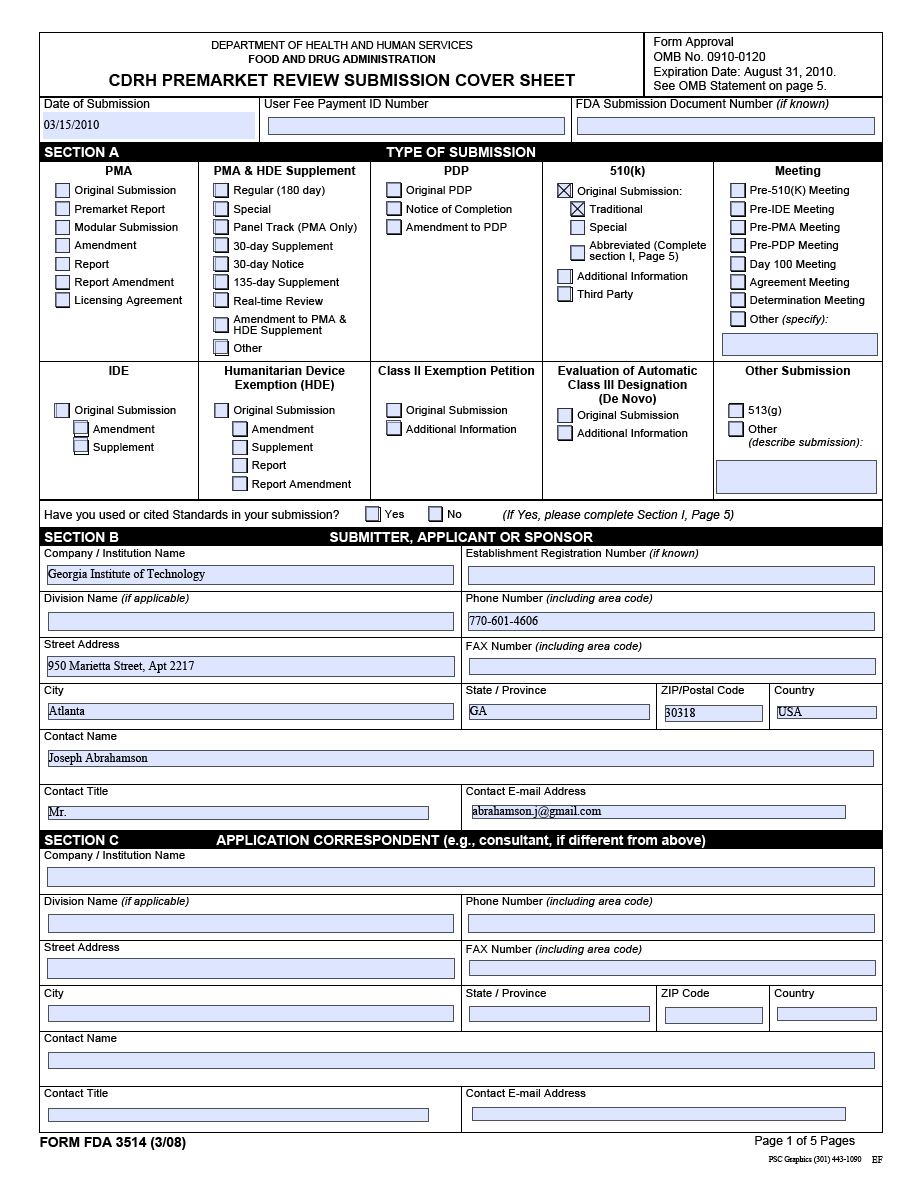
\includegraphics[width=1.2\linewidth]{pages/cdrh-pics/1}
  \label{fig:summary}
\end{figure}

\begin{figure}[H]
  \centering
  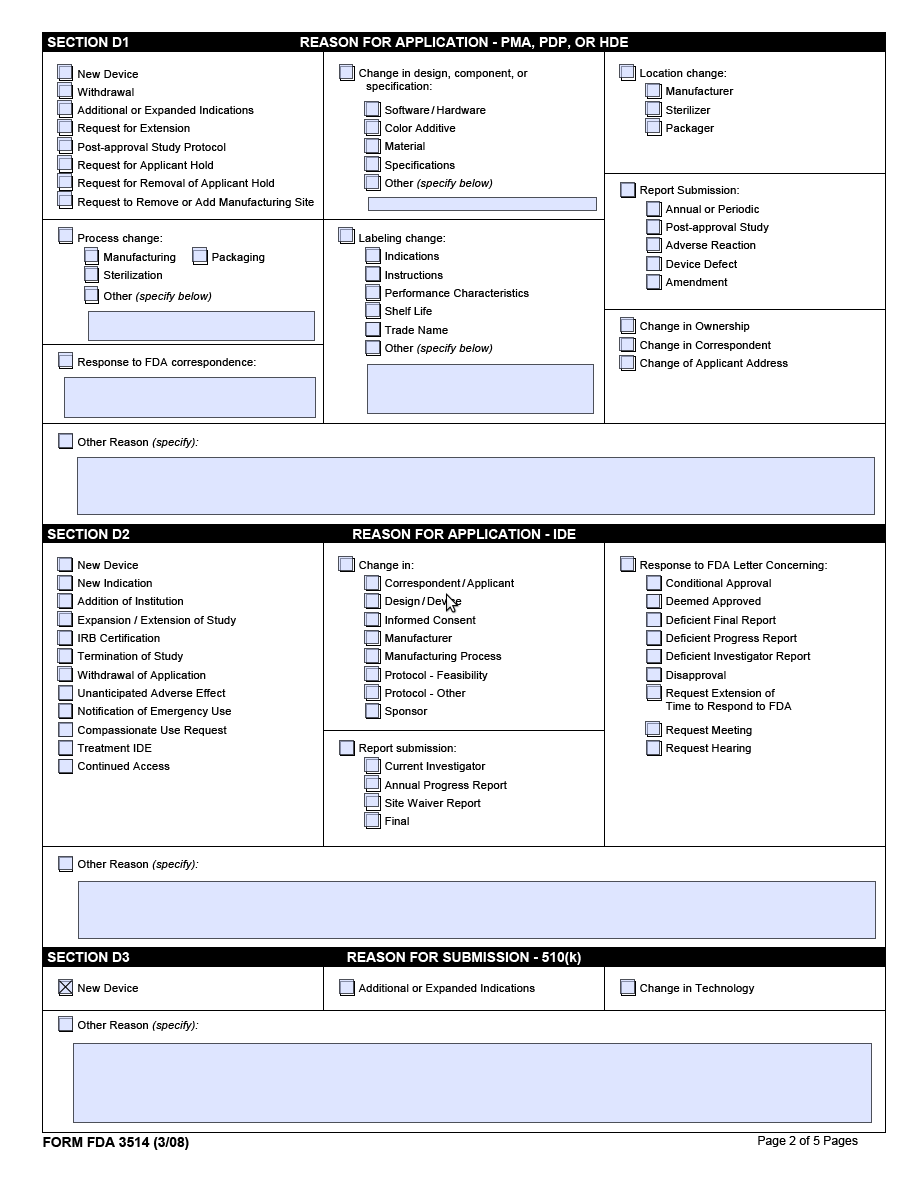
\includegraphics[width=1.2\linewidth]{pages/cdrh-pics/2}
  \label{fig:summary}
\end{figure}

\begin{figure}[H]
  \centering
  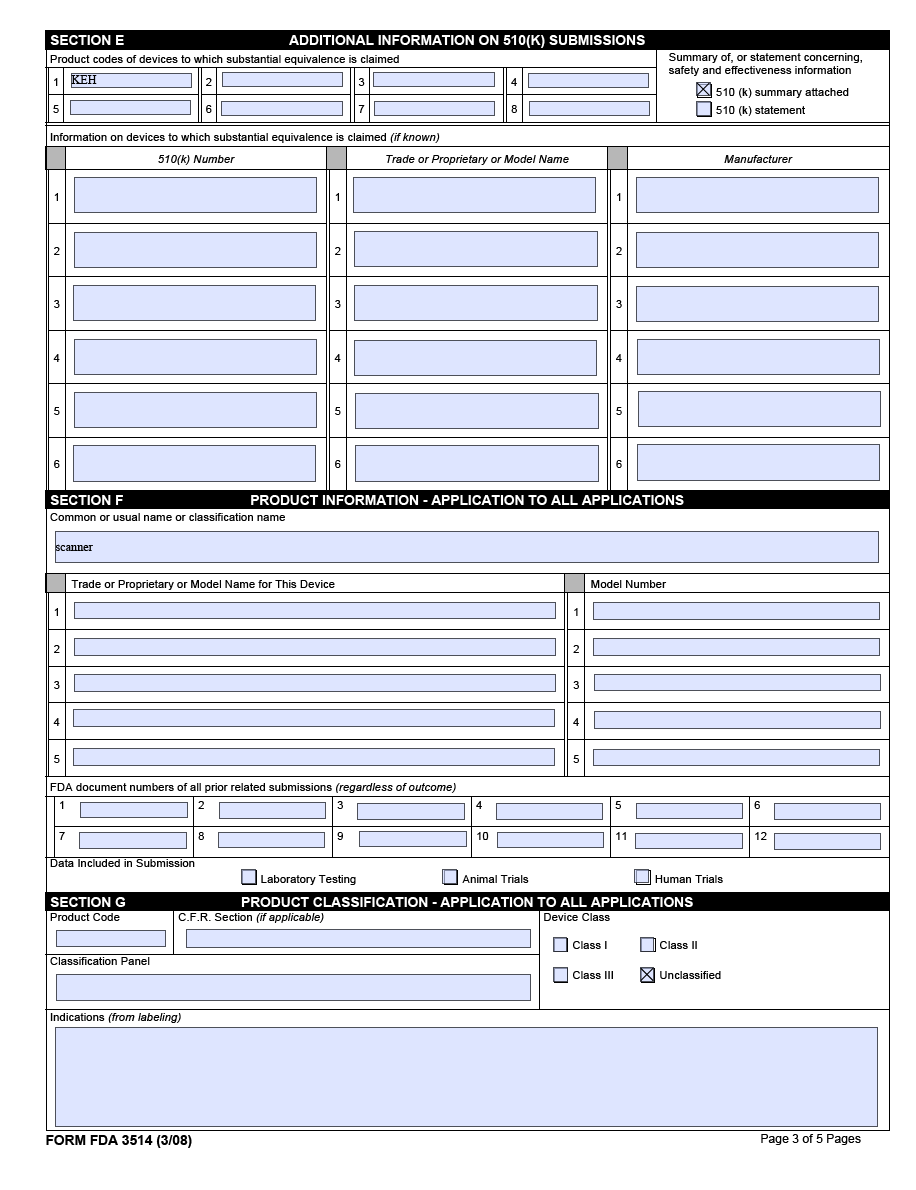
\includegraphics[width=1.2\linewidth]{pages/cdrh-pics/3}
  \label{fig:summary}
\end{figure}

\begin{figure}[H]
  \centering
  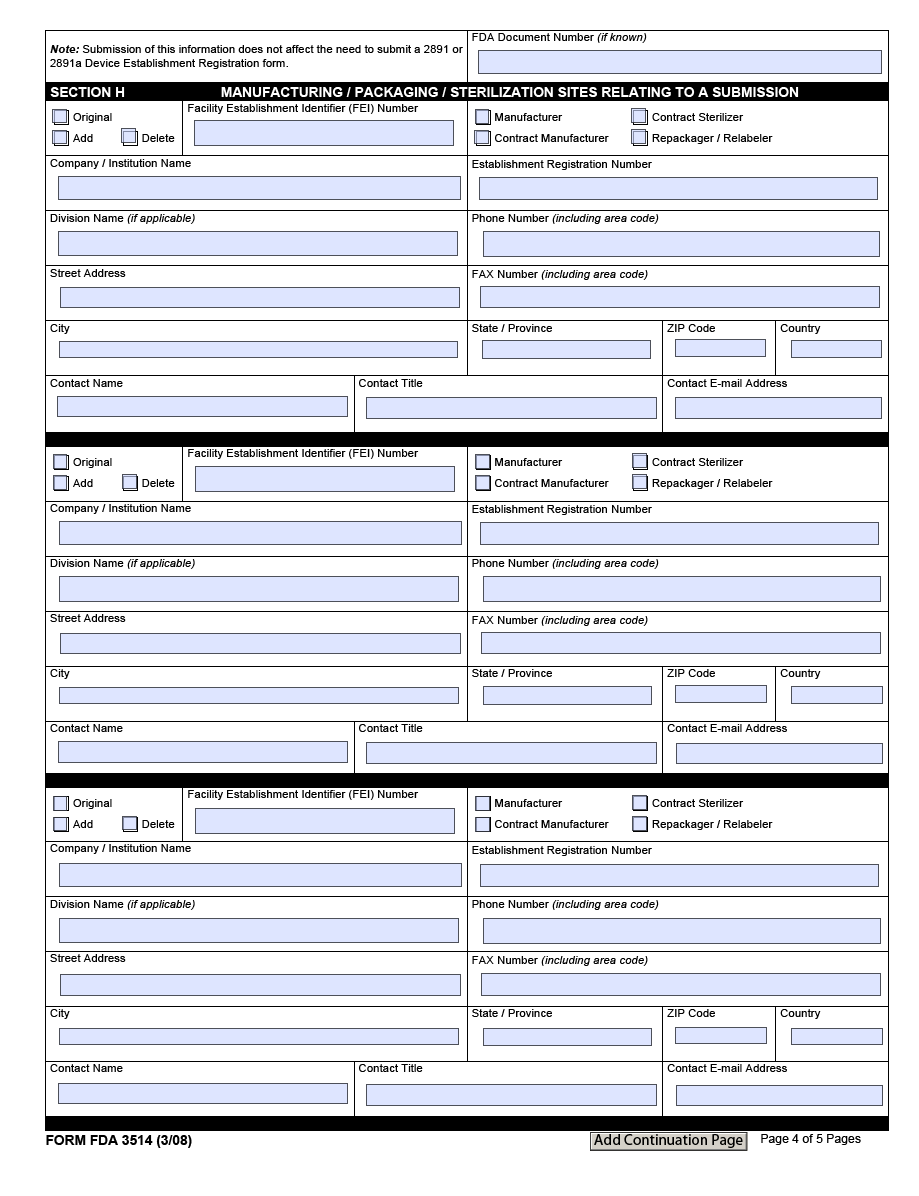
\includegraphics[width=1.2\linewidth]{pages/cdrh-pics/4}
  \label{fig:summary}
\end{figure}

\begin{figure}[H]
  \centering
  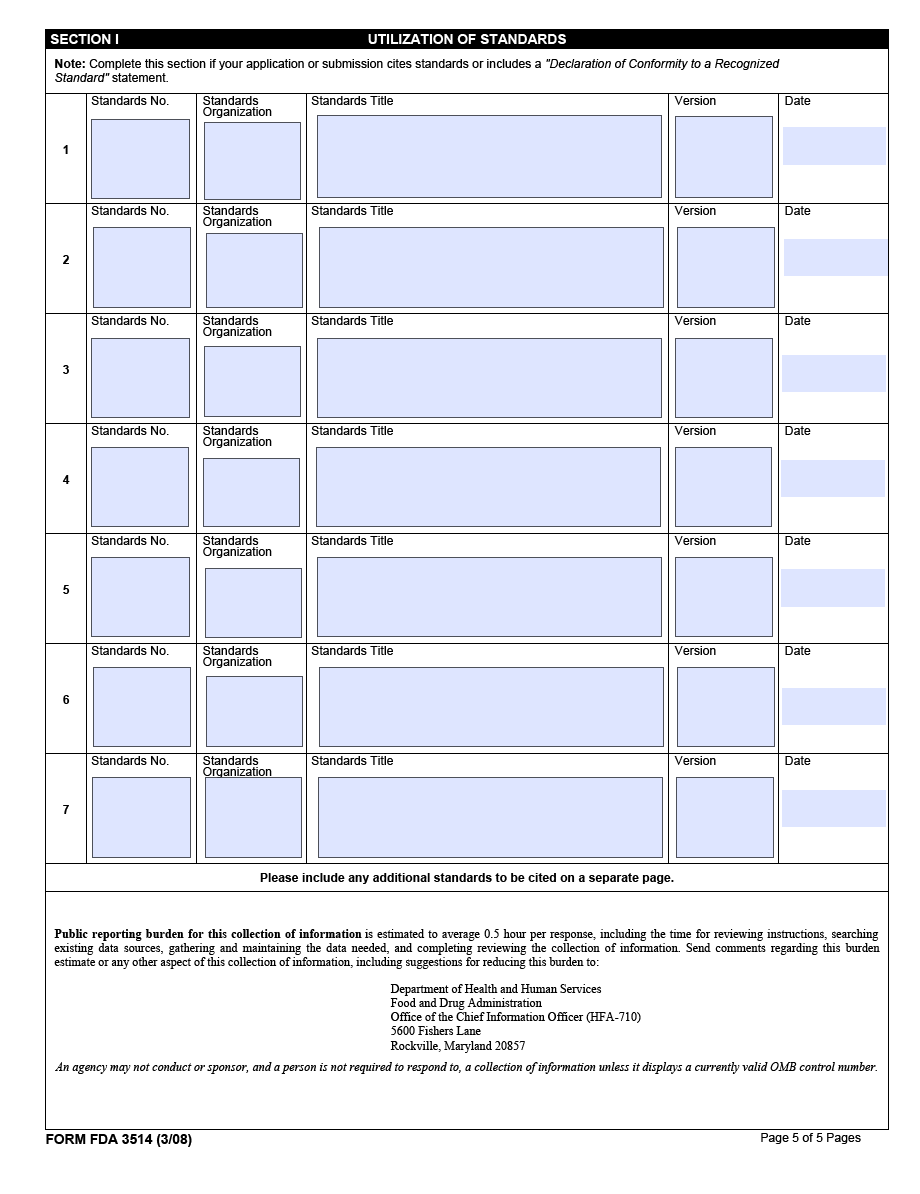
\includegraphics[width=1.2\linewidth]{pages/cdrh-pics/5}
  \label{fig:summary}
\end{figure}

%%% Local Variables: 
%%% mode: latex
%%% TeX-master: "../reg"
%%% End: 

\newpage
\addcontentsline{toc}{subsection}{510(k) Cover Letter}
\singlespacing

\begin{flushright}
  \huge{510(k) Submission --- Traditional}\\[.5in]
  
  \begin{minipage}{0.8\textwidth}
    \begin{flushright}
      \large \textbf{Scanner: eyeScan Mezzo} \\
      \textit{\today}
    \end{flushright}
  \end{minipage}
\end{flushright}

\begin{flushleft}
  Joseph Abrahamson\\
  $<$\textit{abrahamson.j@gatech.edu}$>$ \\
  Phone: 770 601 4606 \\[1em]
  
  \textit{Will register establishment following FDA clearance.}
\end{flushleft}
\vspace{4em}

\onehalfspacing

We seek FDA clearance to market our device, \textbf{eyeScan Mezzo}, a
Class II medical device used for medical scanning of three-dimensional
exterior eye shape. To our knowledge FDA has not classified this
device and, thus, no product code has been assigned or requested for
this device in the Classification Database. Substantially equivalent
devices belong to the General \& Plastic Surgery, Radiology, and
Pathology panels. This finished component is a novel device not
previously marketed with FDA clearance in the USA. We require 510(k)
clearance due to substantial equivalence with existent optical
coherence tomography devices (regulation no. \textbf{886.1570},
product code \textbf{OBO}), x-ray computed tomography devices
(regulation no. \textbf{892.1750}, product code \textbf{JAK}), and
microscopes, micrometers, and accessories (regulation
no. \textbf{864.3600}, product code \textbf{KEH}). Manufacturing
registration is currently unspecified. 

With regards to performance standards, this device contains electrical
components, and is subject to testing under IEC 60601-1-2 Part
I. Furthermore, the device contains a laser component, which under 21
CFR 1000 dictates that the device falls under RCHSA controls. RCHSA
controls indicate that the manufacture of the laser component of this
device is subject to standards 1002.10, 1002.13, and 1002.30, which
specifiy necessary reporting on the manufacturing of the laser
component. Lastly, while the device does contain a laser, it is exempt
from 21 CFR 1040.

%%% Local Variables: 
%%% mode: latex
%%% TeX-master: "../reg"
%%% End:


\newpage
\addcontentsline{toc}{subsection}{Indications for Use Statement}

\begin{center}
  \huge{Indications for Use Statement}\\[.5in]
\end{center}


\onehalfspacing

510(k) Number (if known): N/A \\
Device Name: eyeScan Mezzo \\
Indications for Use: 

%%% Local Variables: 
%%% mode: latex
%%% TeX-master: "../reg"
%%% End: 

\newpage
\addcontentsline{toc}{subsection}{510(k) Statement}
\singlespacing
\begin{center}
  \large{510(k) Statement}
\end{center}

\onehalfspacing


I certify that, in my capacity as product development scientist, I
will make available all information included in this premarket
notification on safety and effectiveness within 30 days of request by
any person if the device described in the premarket notification
submission is determined to be substantially equivalent. The
information I agree to make available will be a duplicate of the
premarket notification submission, including any adverse safety and
effectiveness information, but excluding all patient identifiers, and
trade secret and confidential commercial information, as defined in 21
CFR 20.61.

\begin{figure}[H]
  
\includegraphics[width=0.35\linewidth]{imgs/ja-sig}
\end{figure}

\noindent Joseph Abrahamson \\
\today


%%% Local Variables: 
%%% mode: latex
%%% TeX-master: "../reg"
%%% End: 

\newpage
\addcontentsline{toc}{subsection}{Truthful And Accurate Statement}
\singlespacing
\begin{center}
  \large{Truthful And Accurate Statement}
\end{center}

\onehalfspacing

I certify that, in my capacity as product development scientist, I
believe to the best of my knowledge, that all data and information
submitted in the premarket notification are truthful and accurate and
that no material fact has been omitted.

\begin{figure}[H]
  
\includegraphics[width=0.35\linewidth]{imgs/ja-sig}
\end{figure}

\noindent Joseph Abrahamson \\
\today

%%% Local Variables: 
%%% mode: latex
%%% TeX-master: "../reg"
%%% End: 

\newpage
\addcontentsline{toc}{subsection}{Class I Summary and Certification}
\singlespacing
\begin{center}
  \large{Class I Summary and Certification}
\end{center}

\onehalfspacing

I certify that, in my capacity as product development scientist that I
this device best claims substantial equivalence to a Class I device.

\begin{figure}[H]
  
\includegraphics[width=0.35\linewidth]{imgs/ja-sig}
\end{figure}

\noindent Joseph Abrahamson \\
\today

%%% Local Variables: 
%%% mode: latex
%%% TeX-master: "../reg"
%%% End: 
 % Certified SE to Class I instead of CIII
\newpage
\subsection{Financial Certification or Disclosure Statement}

I certify that, in my capacity as product development scientist that
no clinical studies were performed and thus no financial disclosure is
possible or required.

\begin{figure}[H]
  
\includegraphics[width=0.35\linewidth]{imgs/ja-sig}
\end{figure}

\noindent Joseph Abrahamson \\
\today

%%% Local Variables: 
%%% mode: latex
%%% TeX-master: "../reg"
%%% End: 

\newpage
\subsection{Declarations of Conformity and Summary Reports}

We chose to not rely on a recognized standard or guidance for any part
of the device design or testing. Instead, we have developed a set of
independent testing protocols. Device testing will be conducted using
this independently generated testing protocol and will meet specified
acceptence criteria before the device is marketed. 



% Real sections
\newpage
\setcounter{subsection}{0}
\subsection{Executive Summary}
The device described is a bench top digitizer designed to accurately
measuring the three-dimensional external surface of dissected mouse
eyeballs in research settings. The device is capable of measuring the
mouse eyeballs, held by the optic nerve with inverted tweezers, at a
resolution of \SI{2}{\micro m}. The device utilizes an LED laser
micrometer, two stepper-motor and encoder systems, and a system
controller. 

\newcolumntype{Y}{>{\raggedright\arraybackslash}X}
\begin{figure}[H]
  \begin{tabularx}{\textwidth}{YYYY}
    \toprule
    Characteristics & \mbox{Microscopes} and \mbox{Micrometers} & Optical Coherence \mbox{Tomography} & Computed X-ray \mbox{Tomography} \\ 
    \hline
    Intended Use & x & x &  \\
    \\
    Measurement Approach &   &  & x \\ 
    \\
    Anatomical Site of Interest & & x &  \\
    \\
    Output & & & x \\
    \bottomrule
  \end{tabularx}
  \caption{\textbf{Table of Substantially Equivalent Comparisons:}
    This table compares our device against substantially equivalent
    devices.}
  \label{comparison}
\end{figure}

As indicated in Figure \ref{comparison} there are a few predicate
devices which are claimed as substantially equivalent to the described
device. The similarities between the predicate devices listed and our
device are straightforward to understand. There are a number of key
differences between each listed predicate device and our device. One
recurring difference is that our device is intended solely for use in
research settings, and not for use in medical settings, and especially
not for diagnostic and treatment purposes. Our device is instead
intended for measurement of mouse eyeball specimens in
laboratories. The other key difference is that unlike other
measurement techniques, our device makes use of an LED laser
micrometer to take measurements of the sample.

\newpage
\subsection{Device Description}

The described device (eyeScan Mezzo) is a bench-sized digitizer able
to accurately measure the three-dimensional surface structure of small
organic forms. Specifically designed to measure the convex shape of
dissected mouse eyes down to \SI{2}{\micro m} resolution its likely
usage would involve research aims with respect to eye shape,
morphology, or development especially using genetically modified mouse
models.

In order to achieve these requirements the device must utilize an LED
micrometer, two motor/encoder actuator systems, and a system
controller. The device must be able to accurately position the
micrometer and the loaded object to the \SI{2}{\micro m} level.

Additionally, the device uses a sophisticated loading harness to hold
and rotate the object without needing to account for object
deformation under stress. This harness involves a number of optically
clear pieces and a support polymer.

\newpage
\subsection{Substantial Equivalence Discussion}

\newcolumntype{Y}{>{\raggedright\arraybackslash}X}
\begin{figure}[H]
  \begin{tabularx}{\textwidth}{YYYY}
    \toprule
    Characteristics & \mbox{Microscopes} and \mbox{Micrometers} & Optical Coherence \mbox{Tomography} & Computed X-ray \mbox{Tomography} \\ 
    \hline
    Intended Use & x & x &  \\
    \\
    Measurement Approach &   &  & x \\ 
    \\
    Anatomical Site of Interest & & x &  \\
    \\
    Output & & & x \\
    \bottomrule
  \end{tabularx}
  \caption{\textbf{Table of Substantially Equivalent Comparisons:}
    This table compares our device against substantially equivalent
    devices.}
\end{figure}

\subsubsection{Comparison to Microscopes and Accessories}
Microscopes and accessories are described by the FDA (regulation
number: 864.3600; product code: KEH) as optical instruments used to
enlarge images of specimens, preparations, and cultures for medical
purposes. Our device is similar in the sense that it is an optical
instrument, as it relies on a LED laser to take
measurements. Furthermore, our device is similar in that the sample to
be measured, namely mouse eyeballs, can be classified as a type of
``tissue specimen.''

Our device differs from microscopes in a number of ways. While the
measurement is optical, the method in which the sample is measured is
very different -- unlike microscopes, our devices takes
cross-sectional measurement slices by rotating the sample between the
LED micrometer. Our device also differs in that it further processes
the stack of cross-sectional measurements to generate a
three-dimensional reconstruction of the sample. Our device is also
specifically intended to be used with mouse eyeballs. Lastly, our
device is intended for use only in research settings, whereas
microscopes are allowed for use in medical settings.

\subsubsection{Comparison to Optical Coherence Tomography}
Ophthalmoscopes are described by the FDA (regulation number: 886.1570;
product code: OBO) as diagnostic devices which aid in the detection
and management of various ocular diseases [\ldots] capable of viewing,
imaging, measurement, and analysis of ocular structures. Our device is
similar in that it precisely measures eyeballs and reconstructs their
three dimensional external surface. Our device is clearly focused on
the same anatomical site.

Our device differs from ophthalmoscopes in a number of ways. Unlike
ophthalmoscopes, our device makes measurements using an LED
laser. Furthermore, our device differs in that it also takes
cross-sectional slices by rotating the sample between the LED
micrometer. Additionally, our device differs in that its intended use
is not at all diagnostic in nature. 

\subsubsection{Comparison to X-Ray Computed Tomography}
Our device is similar to x-ray computed tomography systems in that it
makes similar cross-sectional measurements of samples. Our device is
also similar in that involves a similar back-projection based
reconstruction in generating the three dimensional surface of the
measured object. 

Our device is different from x-ray computed tomography systems in that
it uses a laser which emits in the visible spectrum as opposed to
x-ray radiation. Our device is also different in that it is not
intended for medical use, nor for use with live subjects. Our device is
instead intended for use with dissected mouse eyeballs in research
settings.

\newpage
\subsection{Proposed Labeling}

The device labeling will include three general categories: packaging,
marketing copy, and operation manuals. Due to the exception of section
502(f) as orchestrated by part 801.125, the operations manual will be
distributed electronically.

\subsubsection{Packaging}
The device is marketed at an operational research lab and therefore
does not require intensive package marketing. Instead an austere
recycled carboard box tied with twine is labeled simply with the
device name (eyeScan Mezzo) and appropriate device IDs.

\subsubsection{Operations Manual}
The operations manual will consist of an easily accessible electronic PDF document divided
into three subsections. The first will detail the process for making
the solution in which the eyeball is suspended; the second will
describe how to suspend the eyeball in solution; and the third will
consist of instructions for connecting the entire device to a
computer.

The suspension solution is polydimethylsiloxane (PDMS), to be made
using the Sylgard 184 Silicone Elastomer Kit included with the device. 1 gram of base solution
and 0.03 grams of curing agent are to be combined in an optical glass
tube at room temperature using a pipette. The resulting solution is to
be well mixed.

To suspend the eyeball in solution, the eyeball will be rinsed
using aqueous water. Inverted tweezers will be used to pick up the
eyeball by the optic nerve and gently suspend it in the center of the
tube containing polymer solution. The tube will then be capped tightly
and placed into the top slot of the scanning machine.

The device’s user interface will consist of two wires. One wire will
plug into a standard United States outlet of 120 V at 60 Hz and the
other will be a USB cable that plugs into a standard USB drive in a
computer. This will allow the device to transmit scanning data to a
computer for three-dimensional reconstruction. The device will also
have a power on/off switch at the back.

The Sylgard 184 Silicone Elastomer kit will include a brief operations
manual along with MSDS information in paper format.

\subsubsection{Marketing Copy}

\paragraph{Description}
The device, named eyeScan Mezzo, is a bench-sized digitizer able to  and intended to accurately measure and create digital meshes corresponding to the three-dimensional surface structure of dissected rat eyes. It is accurate to a 2 um resolution. EyeScan Mezzo is not intended for use in the diagnosis or treatment of diseases for live animals or humans. Device testing is conducted using developer generated testing protocol and will meet specified acceptance criteria before the device is marketed. Full testing of the device's EMC characteristics is performed according to IEC 60601-1-2 Part I.

\paragraph{Safety and Effectiveness Considerations}

EyeScan Mezzo is intended to be operated only by trained laboratory personnel in ophthalmological research settings only. It poses no known immediate health hazard to the operator. 

\paragraph{Contraindications, Warnings, Precautions}

PDMS is toxic to humans, and as such, contact with skin and organs should be avoided. If PDMS does come into contact with the skin, eyes, or body, one should immediately clean off PDMS from body part using a paper towel and rinse contaminated area under running water. Refer to the MSDS for further instruction.

Insertion of objects other than that indicated in the operations manual may damage the device.
If any foreign object enters the device, the operator should turn off the device and cut off the power supply to the device immediately. The operator should then remove the protection casing of the device, remove the foreign object, and reinstall the protection casing. If the device is damaged to the point of malfunction, the operator should contact the manufacturer for repairs. 

A liquid spill inside the machine may damage electronic components and pose an electrical hazard.
If a liquid spill occurs, the operator should turn off the device and cut off the power supply to the device immediately. The operator should then send in a request to the manufacturer to replace damaged parts.

Proper laboratory attire such as latex gloves, laboratory coats, and goggles should be worn before operating the device. 

Injury may result if the device is operated by untrained personnel. 


%%% Local Variables: 
%%% mode: latex
%%% TeX-master: "../reg"
%%% End: 

\newpage
\newpage
\subsection{Sterilization and Shelf Life}

This device is not sold as sterile. During operation, sterility
does not impact the safety of effectiveness of the device.

\newpage
\newpage
\subsection{Biocompatibility}

This device contains no components which come into direct or indirect
contact with patients. The device is intended for use in research
settings, not clinical settings.

Furthermore, we claim substantial equivalence with microscopes and
accessories (regulation number: 864.3600, product code:
KEH). Microscopes and accessories are identified as optical
instruments used to enlarge images of specimens, preperations, and
cultures for medical purposes. Our device thus makes use of identical
materials used in devices claimed to be substantially equivalent, as
it is intended for use with dissected eyeballs. 

\newpage
\subsection{Software}

The software elements in the described device are considered to be of
\textit{minor regulatory concern} since neither the device nor the
output of its software can in any way, direct or indirect, cause harm
to operators or patients or deliver information useful in a medical
diagnosis. The software involved with this device includes control and
automation firmware for the motion of the device's frame, recording
and reconstruction algorithms for interpreting data from the
micrometer, and standalone software on a general purpose computer for
control and viewing of the reconstructed meshes.

The device is non-hazardous in that neither the operator nor the
patient have any contact, direct or indirect, with the device while it
is operational.

The software requirements involve three stages: automation,
reconstruction, and control. 

\begin{itemize}
\item The \textit{automation} section is required to accurately
  control position of the measured piece and the micrometer within the
  device while maintaining accurate real-time position information from
  the motor encoders. This section will be written in National
  Instrument's (NI) LabView Real-time and compiled to very-high-speed
  integrated circuit hardware description language (VHDL) and deployed
  on an NI Reprogrammable Input Output (RIO) device.
\item The \textit{reconstruction} section is required to produce
  online reconstructions of the measured data in a format readable
  offline. This is instrumental in troubleshooting the usage of the
  device during the scan and must also be carefully implemented to
  prevent distortions. This section will be programmed partly in
  LabView Real-time for any real-time processing as to be deployed on
  the RIO and then completed in compiled C on the general purpose
  platform.
\item The \textit{control} section is the standalone software deployed
  on a general purpose computer and in communication with the
  device. This software both allows real-time feedback to the operator
  from the device and also allows for sequence programming and
  control. This section will be programmed in Python and deployed on
  the general purpose computer platform.
\end{itemize}

The functional software testing and validation are largely functional
and have been previously specified in the previous Testing and
Verification Protocol document. Current testing status has not yet
reached the software level and therefore no results yet exist. The
Testing and Verification Protocol document is available at request.
\newpage
\subsection{Electromagnetic Compatibility and Electrical Safety}

Our device does contain a number of sensitive electronic
devices. Electrical failure of the device cannot result in safety
hazards as under electrical interference the device will simply fail
to deliver results. Additionally, the components of the device are
hardened to electrical shock and resonance. Full testing of the
device's EMC characteristics will be performed according to IEC
60601-1-2 Part I.

There is no patient contact with electrical components of the device
as the device is intended to be used exclusively with dissected
eyeballs in research settings.


%%% Local Variables: 
%%% mode: latex
%%% TeX-master: "../reg"
%%% End: 


%\subsection{Performance Testing --- Lab, Animal, Clinical}
% Not required


\newpage
\addcontentsline{toc}{section}{References}
\bibliographystyle{unsrt}
\bibliography{../tex/bibl}

\end{document}
%%% Local Variables: 
%%% mode: latex
%%% TeX-master: t
%%% End: 
